\documentclass[12pt, a4paper]{article}

\usepackage{amsmath}
\usepackage{bbm}
\usepackage{amsfonts}
\usepackage{graphicx}
\usepackage{pdfpages}
\usepackage[titletoc, title]{appendix}
\usepackage{hyperref}
\hypersetup{
    colorlinks=true,
    linkcolor=blue,
    filecolor=magenta,      
    urlcolor=cyan,
}


\def\va{\boldsymbol{a}}
\def\vb{\boldsymbol{b}}
\def\vc{\boldsymbol{c}}
\def\vh{\boldsymbol{h}}
\def\vs{\boldsymbol{s}}
\def\vw{\boldsymbol{w}}
\def\vx{\boldsymbol{x}}
\def\vy{\boldsymbol{y}}
\def\vz{\boldsymbol{z}}
\def\v1{\boldsymbol{1}}

\def\vI{\boldsymbol{I}}
\def\vR{\boldsymbol{R}}
\def\vU{\boldsymbol{U}}
\def\vV{\boldsymbol{V}}
\def\vW{\boldsymbol{W}}
\def\vX{\boldsymbol{X}}
\def\vY{\boldsymbol{Y}}

\def\vtheta{\boldsymbol{\theta}}

\def\rmx{\mathrm{x}}

\def\vrmx{\boldsymbol{\mathrm{x}}}
\def\vrmy{\boldsymbol{\mathrm{y}}}
\def\vrmX{\boldsymbol{\mathrm{X}}}
\def\vrmY{\boldsymbol{\mathrm{Y}}}

\def\E{\mathbb{E}}
\def\X{\mathbb{X}}
\def\R{\mathbb{R}}

\def\st{\textit{s.t.}}

\DeclareMathOperator*{\relu}{ReLU}
\DeclareMathOperator*{\argmax}{arg\,max}
\DeclareMathOperator*{\argmin}{arg\,min}
\DeclareMathOperator*{\softmax}{softmax}
\DeclareMathOperator*{\diag}{diag}

\newcommand{\egva}[1]{\boldsymbol{a}^{(#1)}}
\newcommand{\egvb}[1]{\boldsymbol{b}^{(#1)}}
\newcommand{\egvc}[1]{\boldsymbol{c}^{(#1)}}
\newcommand{\egvg}[1]{\boldsymbol{g}^{(#1)}}
\newcommand{\egvh}[1]{\boldsymbol{h}^{(#1)}}
\newcommand{\egvo}[1]{\boldsymbol{o}^{(#1)}}
\newcommand{\egvs}[1]{\boldsymbol{s}^{(#1)}}
\newcommand{\egvx}[1]{\boldsymbol{x}^{(#1)}}
\newcommand{\egvy}[1]{\boldsymbol{y}^{(#1)}}
\newcommand{\egvU}[1]{\boldsymbol{U}^{(#1)}}
\newcommand{\egvV}[1]{\boldsymbol{V}^{(#1)}}
\newcommand{\egvW}[1]{\boldsymbol{W}^{(#1)}}
\newcommand{\egh}[1]{h^{(#1)}}
\newcommand{\ego}[1]{o^{(#1)}}
\newcommand{\egx}[1]{x^{(#1)}}
\newcommand{\egy}[1]{y^{(#1)}}
\newcommand{\egL}[1]{L^{(#1)}}
\newcommand{\eghy}[1]{\hat{y}^{(#1)}}
\newcommand{\eghvy}[1]{\hat{\boldsymbol{y}}^{(#1)}}

\newcommand{\expect}[3]{\mathbb{E}_{#1 \sim #2} \left[ #3 \right]}
\newcommand{\dkl}[2]{D_{\mathrm{KL}}(#1 \Vert #2)}
\newcommand{\condiP}[3]{P(#1 \mid #2;#3)}
\newcommand{\condip}[3]{p(#1 \mid #2;#3)}
\newcommand{\ND}[3]{\mathcal{N}(#1;#2,#3)}

\newcommand{\dx}[1]{\frac{\mathrm{d}}{\mathrm{d}x} #1}
\newcommand{\pard}[2]{\frac{\partial #1}{\partial #2}}
\newcommand{\tpard}[2]{\left(\frac{\partial #1}{\partial #2}\right)^\top}


\title{Recurrent Neural Network}
\author{CHEN Si}
\date{}


\begin{document} 


\maketitle
\tableofcontents


\section{Definition}
\begin{center}
    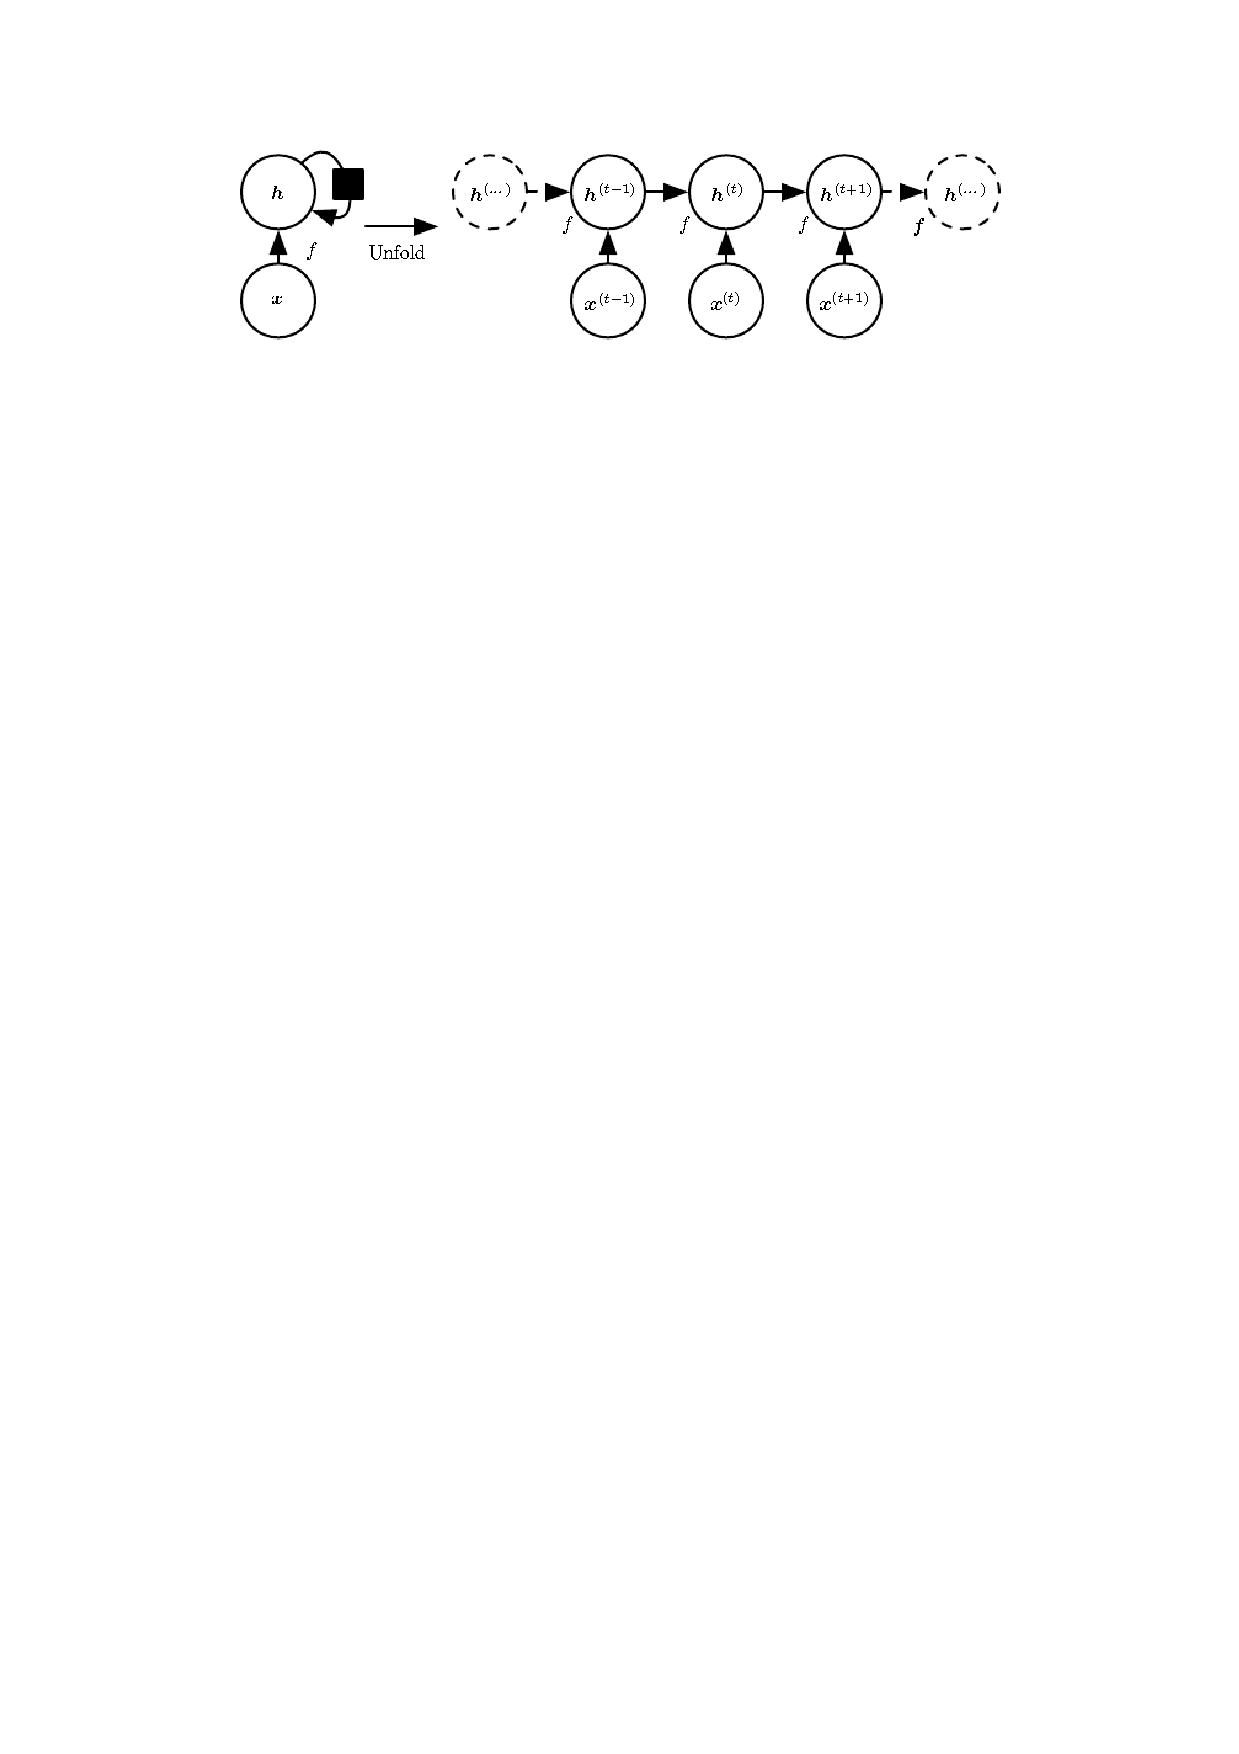
\includegraphics[width=0.9\textwidth]{../imgs/Recurrent_Network_without_Outputs.pdf}
\end{center}
\[
    \egvh{t} = f(\egvh{t-1}, \egvx{t};\vtheta)
\]
\begin{itemize}
    \item Hidden units $\vh$ represents
        \begin{enumerate}
            \item the state of the dynamical system.
            \item lossy summary of the task-relevant aspects of the past sequence of inputs up to $t$, when the recurrent network is trained to perform a task that requires predicting the future from the past.
        \end{enumerate}
    \item Black square indicates that an interaction takes place with a delay of a single time step.
\end{itemize}


\subsection{Motivation}

\paragraph{Dynamical System}
\subparagraph{Unfolded Computational Graph}
\begin{center}
    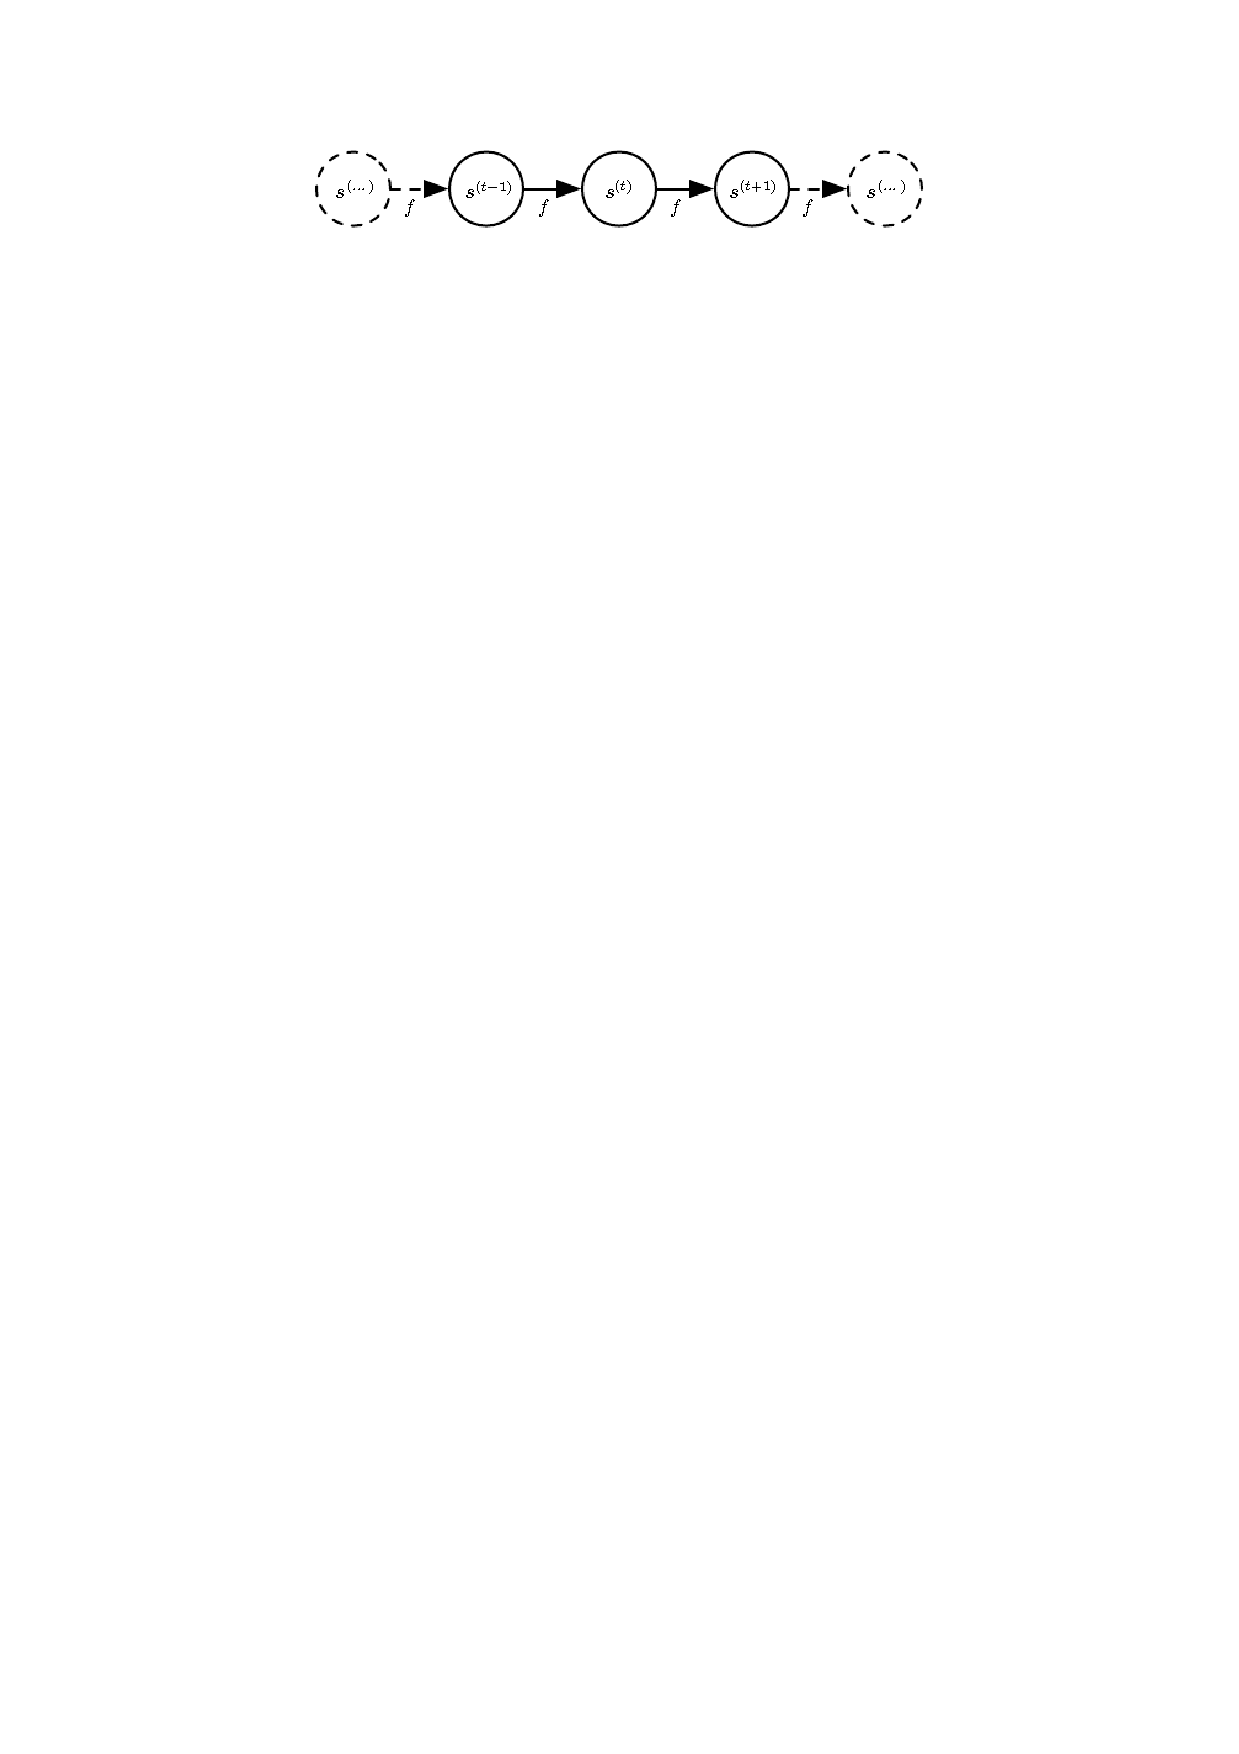
\includegraphics[width=0.8\textwidth]{../imgs/Dynamical_System.pdf}
\end{center}
where $\egvs{t}$ is called the \textbf{state} of the system.
\subparagraph{Recurrent Defintion}
\[
    \egvs{t} = f(\egvs{t-1};\vtheta)
\]
\subparagraph{Unfolded Definition (up to step 3)}
\[
    \begin{split}
        \egvs{3} &= f(\egvs{2};\vtheta)
        \\&= f(f(\egvs{1};\vtheta);\vtheta)
    \end{split}
\]

\paragraph{Dynamical System with External Signal $\egvx{t}$}
\[
    \egvs{t} = f(\egvs{t-1}, \egvx{t}; \vtheta)
\]


\subsection{Advantages}
\begin{enumerate}
    \item Learning just a single model $f$:
        \begin{itemize}
            \item The learned model always has the same input size, regardless of the sequence length.
            \item Parameter sharing: It is possible to use the same transition function $f$ with the same parameters at every time step.
            \item Allows generalization to sequence lengths that does not appear in the training set.
            \item Requires much fewer training examples to estimate.
        \end{itemize}
\end{enumerate}


\subsection{Disadvantages}
\begin{enumerate}
    \item Optimizing the parameters may be difficult, because of the reduced number of parameters.
\end{enumerate}


\subsection{How to determine the length $\tau$}
\begin{enumerate}
    \item Add a special symbol corresponding to the end of a sequence.
    \item Introduce an extra Bernoulli output to the model that represents the decision to either contnue generation or halt generation at each time step. (a more general way)
    \item Add an extra output to the model that predicts the interger $\tau$ itself.
        \[
            P(\egvx{1},\dots,\egvx{\tau}) = P(\tau) P(\egvx{1},\dots,\egvx{\tau} \mid \tau)
        \]
\end{enumerate}


\section{Taxonomy}

\subsection{Sequence to Sequence of the same length}

\subsubsection{}
Recurrent networks that produce an output at each time step and have recurrent connections between hidden units.
\begin{equation}
    \begin{split}
        \egva{t} &= \vb + \vW\egvh{t-1} + \vU\egvx{t} \\
        \egvh{t} &= \tanh(\egva{t}) \\
        \egvo{t} &= \vc + \vV\egvh{t} \\
        \eghvy{t} &= \softmax(\egvo{t})
    \end{split}
    \label{rnn_for}
\end{equation}
with a initial state $\egvh{0}$.
\begin{center}
    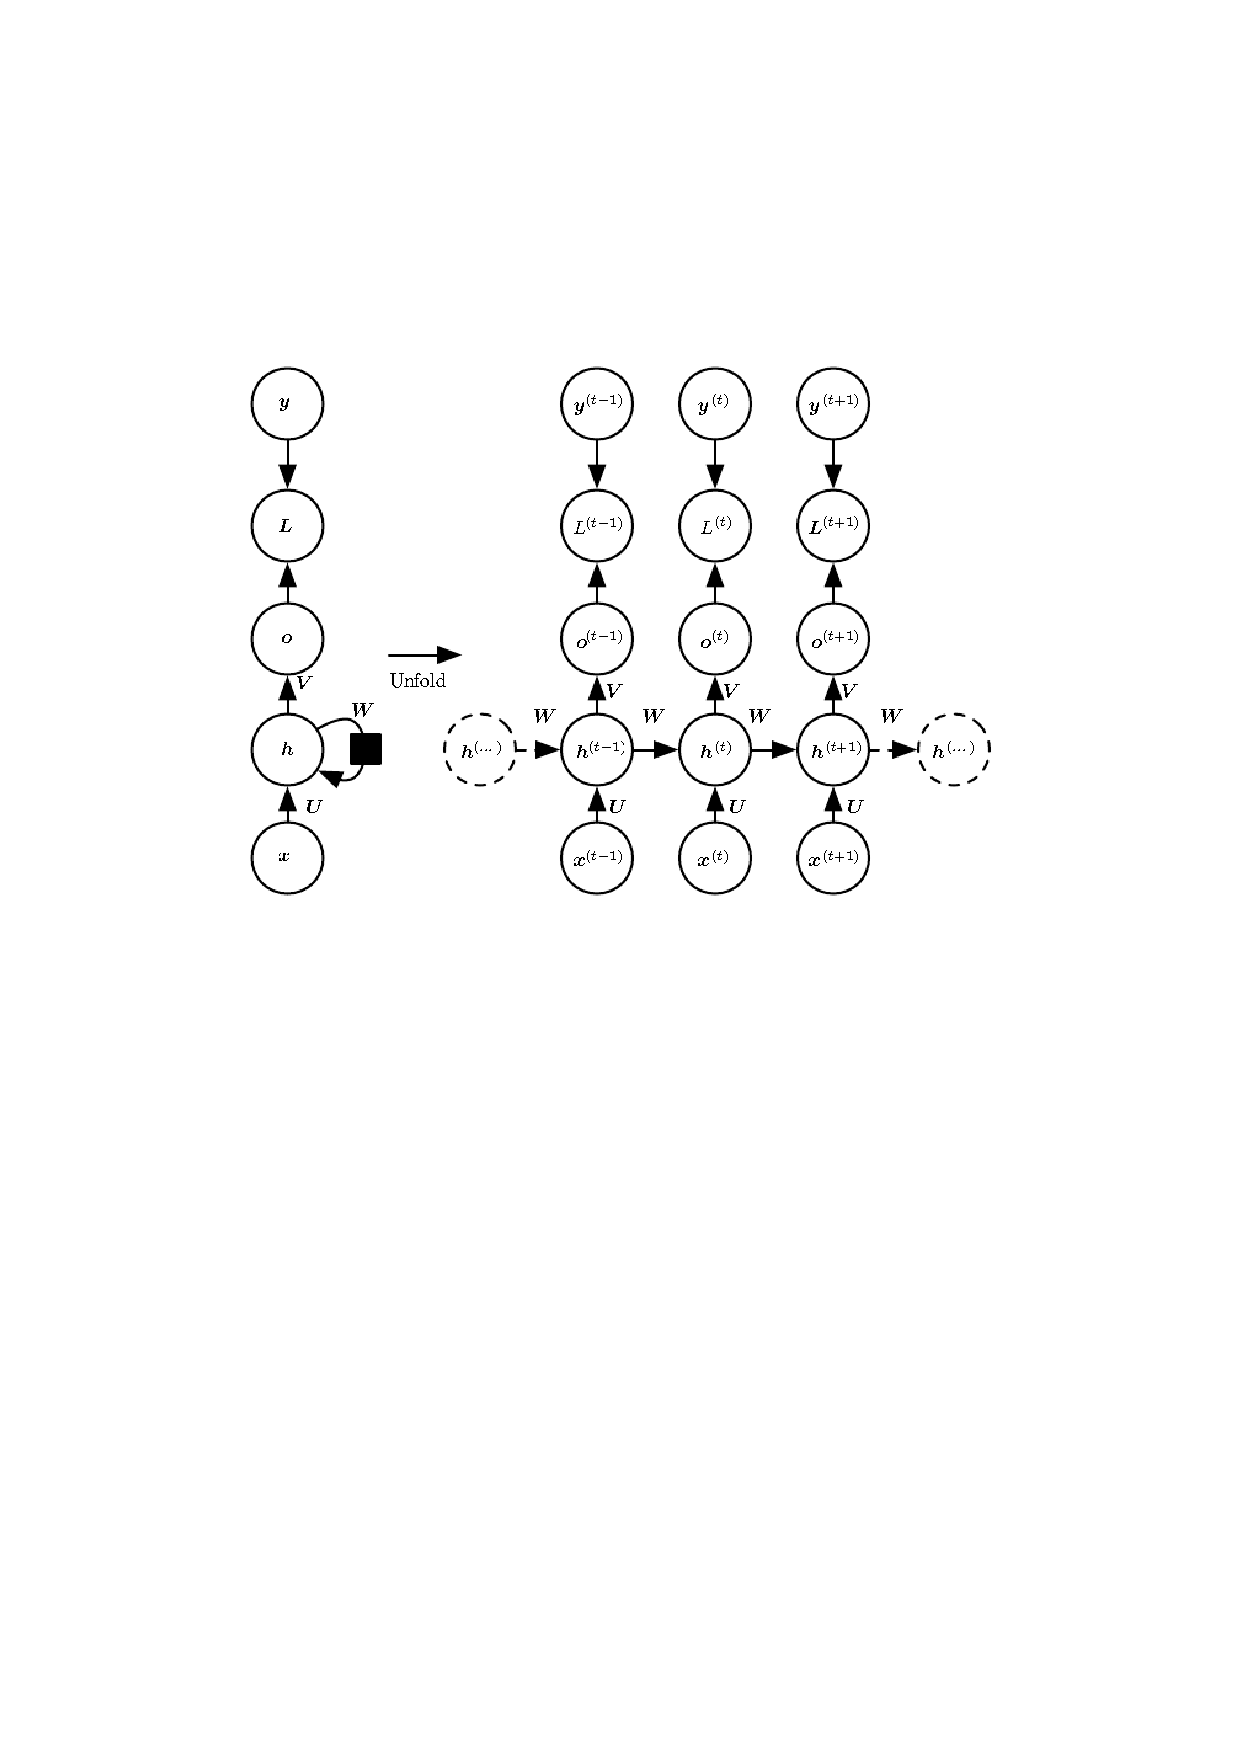
\includegraphics[width=0.9\textwidth]{../imgs/RNN_1.pdf} 
\end{center}

\paragraph{Characteristics}
\begin{itemize}
    \item Maps an input sequence to an output sequence of the same length.
    \item{
        Loss:
        \begin{equation}
            \begin{split}
                & L\left( \{\egvx{1},\dots,\egvx{\tau}\}, \{\egvy{1},\dots,\egvy{\tau}\} \right)
                \\=& \sum_t \egL{t}
                \\=& - \sum_t \log p_\text{model} \left( \egy{t} \mid \{\egvx{1},\dots,\egvx{t}\} \right)
            \end{split}
            \label{rnn_loss}
        \end{equation}
        where $\egL{t}$ is the negative log-likelihood of $\egy{t}$ given $\egvx{1},\dots,\egvx{t}$
        \begin{itemize}
            \item{
                Conditional independence assumption: The conditional distribution 
                \[
                    P( \egvy{1},\dots,\egvy{\tau} \mid \egvx{1},\dots,\egvx{\tau} ) = 
                    \prod_t P(\egvy{t} \mid \egvx{1},\dots,\egvx{t})
                \]
            }
        \end{itemize}
    }
    \item Runtime is $O(\tau)$, memory cost is $O(\tau)$.
    \item Only able to represent distributins in which the $\vy$ values are conditionally independent from each other given the $\vx$ values.
\end{itemize}

\subsubsection{}
Recurrent networks that produce an output at each time step and have recurrent connections only from the output at one time step to the hidden units at the next time step.
\begin{center}
    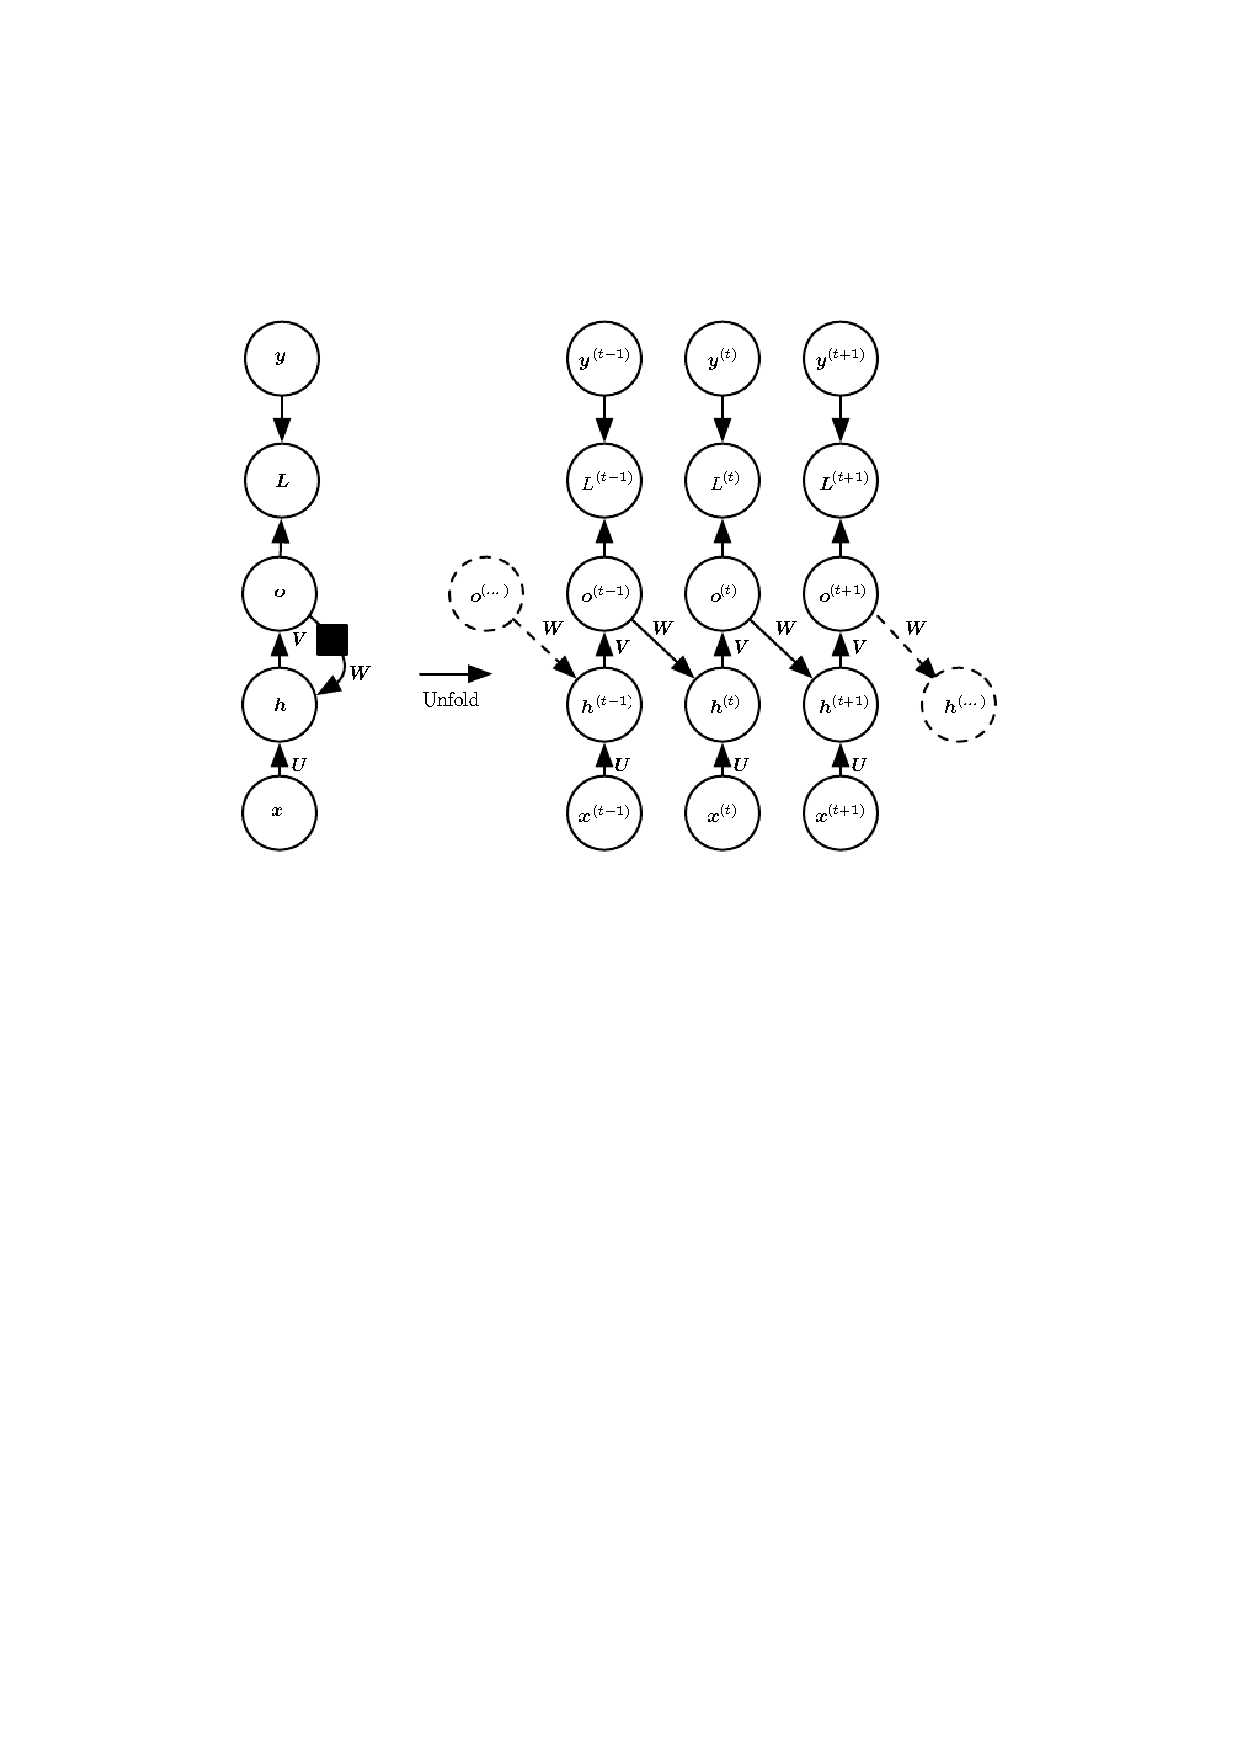
\includegraphics[width=0.9\textwidth]{../imgs/RNN_2.pdf}
\end{center}
\paragraph{Characteristics}
\begin{itemize}
    \item Strictly less powerful because it lacks hidden-to-hidden recurrent connections. (e.g. it connot simulate a universal Turing machine.)
    \item Training can be \textbf{parallelized} because all the time steps are decoupled (the training set provides the ideal value of previous output).
    \item Avoids back-propagation through time.
    \item Teacher forcing:
        For example, for a sequence with two time steps
        \[
            \begin{split}
                &\log p\left( \egvy{1},\egvy{2} \mid \egvx{1},\egvx{2} \right)
                \\=& \log p\left(\egvy{2} \mid \egvy{1},\egvx{1},\egvx{2} \right) + \log p\left( \egvy{1} \mid \egvx{1},\egvx{2} \right)
            \end{split}
        \]
        \begin{center}
            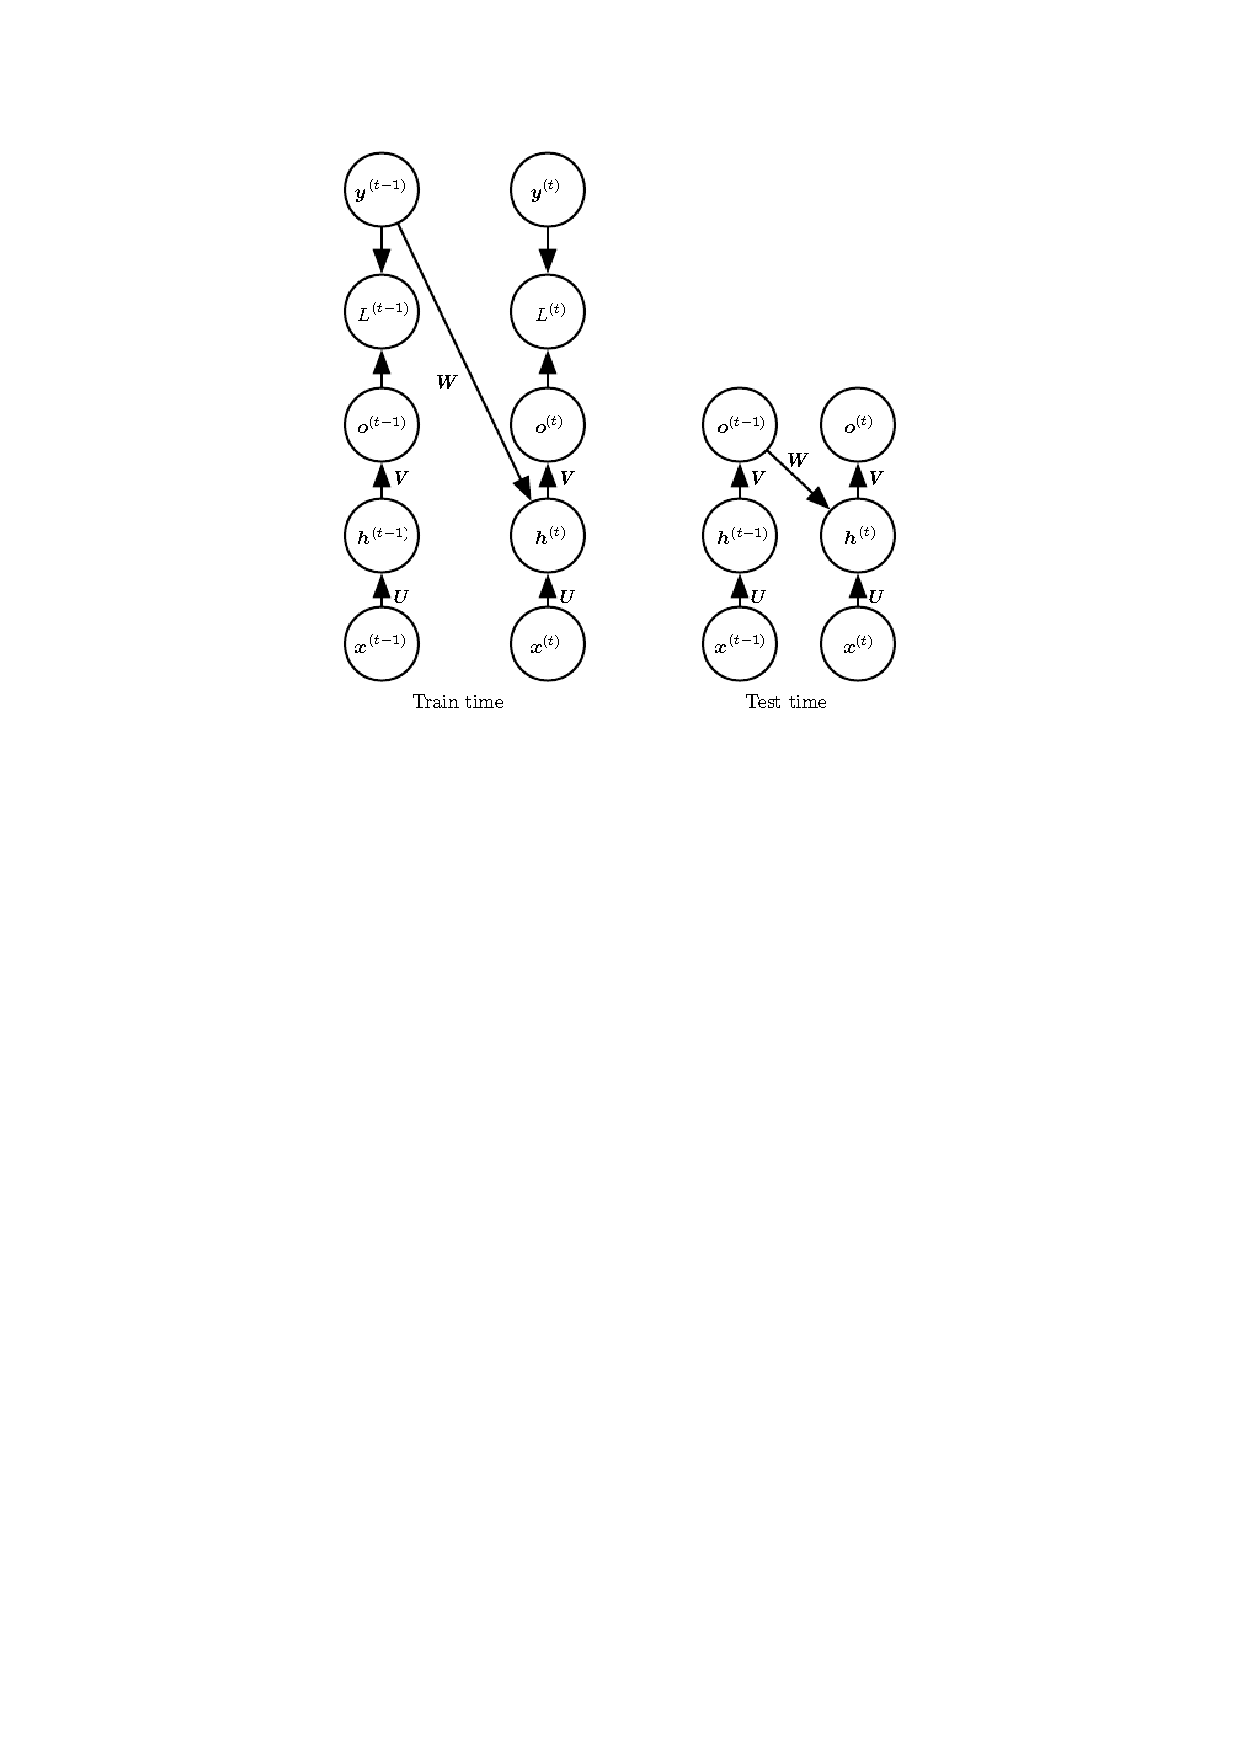
\includegraphics[width=0.7\textwidth]{../imgs/Teacher_Forcing.pdf}
        \end{center}
\end{itemize}
\paragraph{Disadvantages}
\begin{enumerate}
    \item The disadvantages of strict teacher forcing (no BPTT) is that the inputs during training could be quite different from the inputs during testing (\textbf{closed-loop} mode).
        \newline Solutions:
        \begin{enumerate}
            \item Train with both teacher-forced inputs and free-running inputs
            \item Randomly chooses to use generated values or actual data values as input (curriculum learning strategy: gradially use more of the generated values as input).
        \end{enumerate}
\end{enumerate}


\subsubsection{}
\begin{center}
    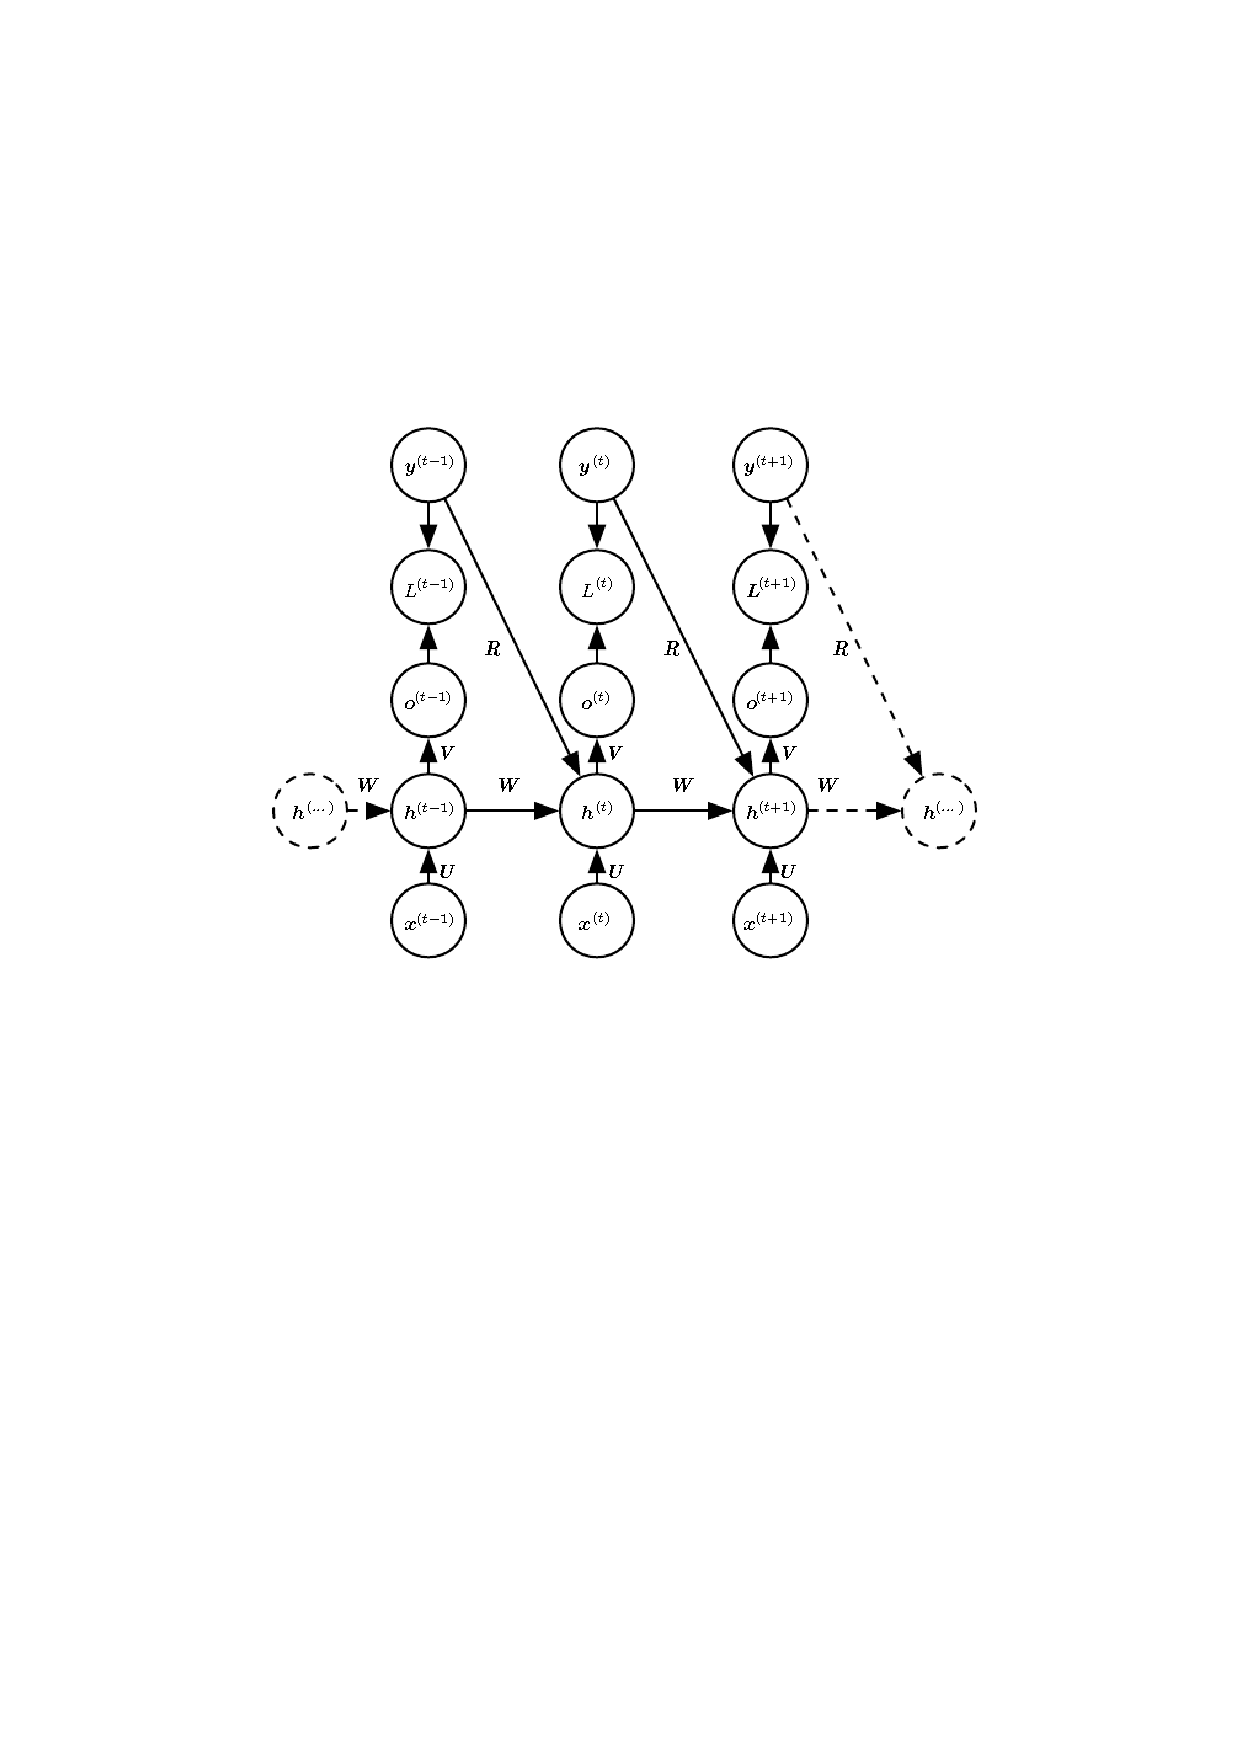
\includegraphics[width=0.9\textwidth]{../imgs/RNN_5.pdf}
\end{center}
\paragraph{Characteristics}
\begin{itemize}
    \item Because of connections from the output at time $t$ to the hidden unit at time $t+1$, the model can represent arbitrary probability distributions over the $\vy$ sequence (no conditional independence assumption).
\end{itemize}
\paragraph{Restrictions}
\begin{enumerate}
    \item The length of both sequences must be the same.
\end{enumerate}


\subsection{Sequence to Fixed-Size Vector}
\subsubsection{}
Recurrent networks with recurrent connections between hidden units, that read an entire sequence and then produce a single output.
\begin{center}
    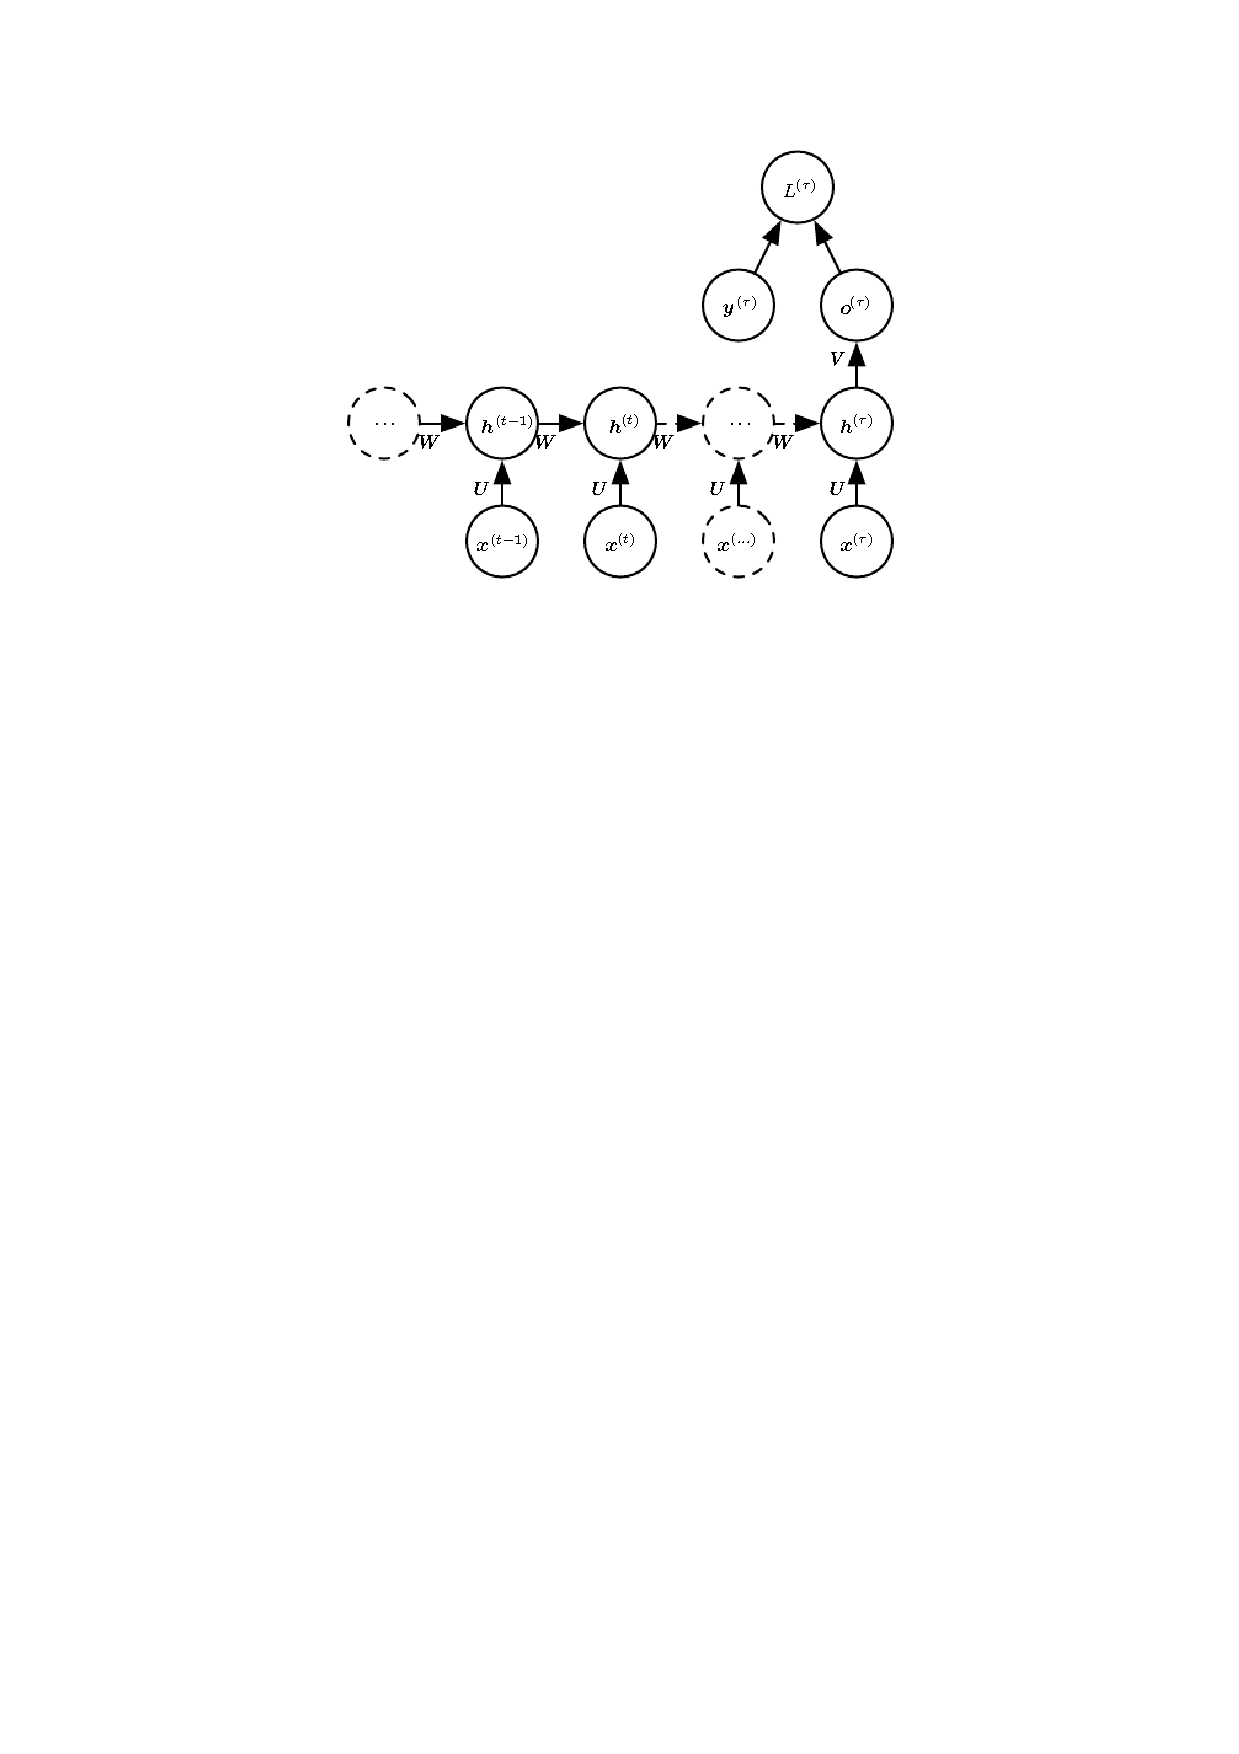
\includegraphics[width=0.9\textwidth]{../imgs/RNN_3.pdf}
\end{center}
\paragraph{Characteristics}
\begin{itemize}
    \item There might be a target right at the end, or the gradient on the ouput $\egvo{t}$ can be obtained by back-propagating from further downstream modules.
\end{itemize}
\paragraph{Applications}
\begin{enumerate}
    \item Summarize a sequence and produce a fixed-size representation used as input for further processing.
\end{enumerate}


\subsection{Fixed-Size Vector to Sequence}
\subsubsection{}
\begin{center}
    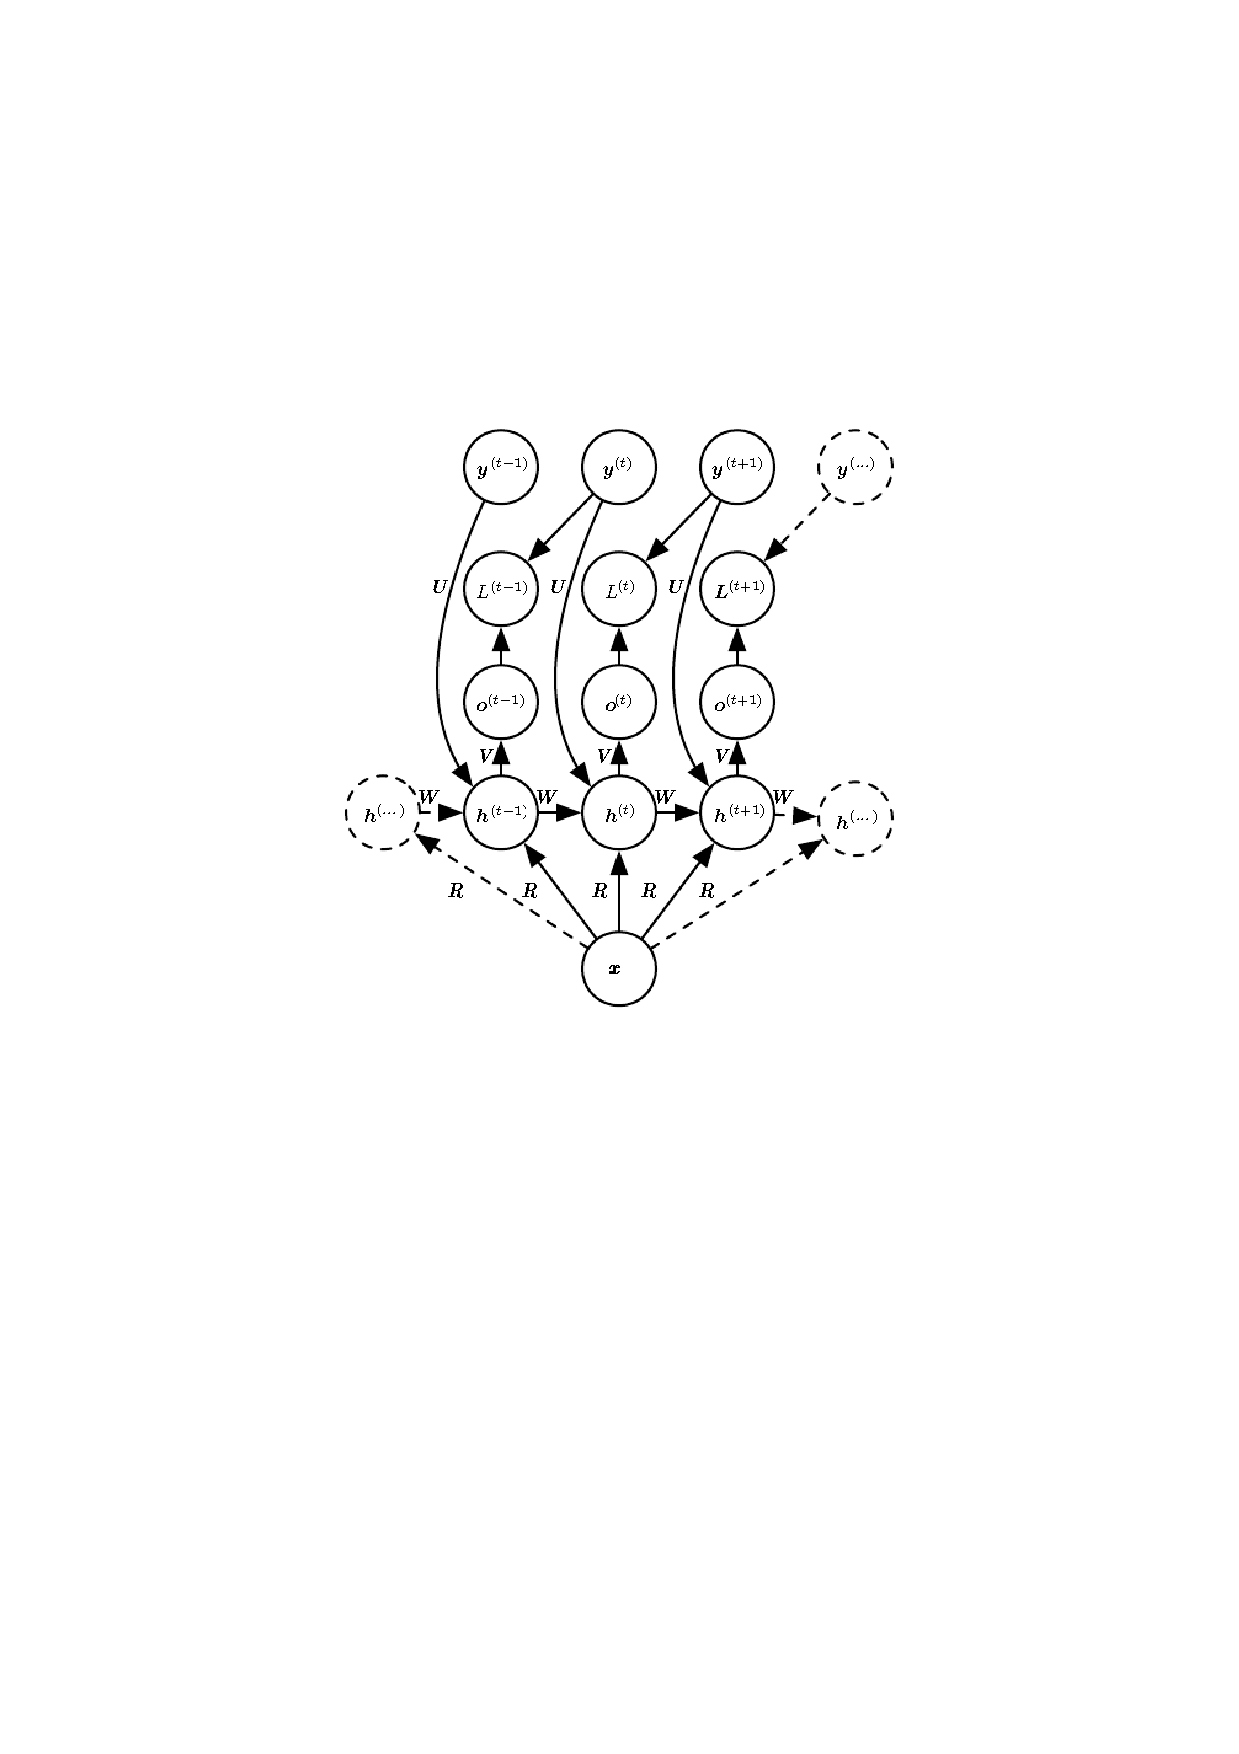
\includegraphics[width=0.9\textwidth]{../imgs/RNN_4.pdf}
\end{center}
\paragraph{Characteristics}
\begin{itemize}
    \item $\vx^\top \vR$ is effectively a new bias parameter.
    \item Each element $\egvy{t}$ of the observed output sequence serves both as input (for the current time step) and, during training, as target (for the previous time step).
\end{itemize}
\paragraph{Applications}
\begin{enumerate}
    \item Image captioning, where a single image is used as input to a model that then produces a sequence of words describing the image.
\end{enumerate}


\section{Back Propagation Through Time (BPTT)}
Here we talk about the BPTT of equation \ref{rnn_for} as forward propagation and equation \ref{rnn_loss} as loss function.
(Note: here $\eghvy{t} = \softmax(\egvo{t})$)
\begin{enumerate}
    \item $\displaystyle \pard{L}{\egL{t}} = 1$
    \item $\displaystyle \left( \nabla_{\egvo{t}} L \right)_i 
        = \pard{L}{\ego{t}_i} 
        = \pard{L}{\egL{t}} \pard{\egL{t}}{\ego{t}_i} 
        = \eghy{t}_i - \mathbbm{1}_{i=\egy{t}}$
    \item For $t=\tau$
        \[
            \nabla_{\egvh{\tau}}L = \vV^\top \nabla_{\egvo{\tau}} L  
        \]
        $\forall t = 1,\dots,\tau-1$
        \[
            \begin{split}
                \nabla_{\egvh{t}}L 
                &= \left( \pard{\egvh{t+1}}{\egvh{t}} \right)^\top (\nabla_{\egvh{t+1}}L) 
                + \left( \pard{\egvo{t}}{\egvh{t}} \right)^\top (\nabla_{\egvo{t}}L)
                \\&= \vW^\top \diag\left( 1-\left(\egvh{t+1}\right)^2 \right)(\nabla_{\egvh{t+1}}L) + \vV^\top(\nabla_{\egvo{t}}L)
            \end{split}
        \]
    \item
        \[
            \begin{split}
                \nabla_{\vc}L &\quad=\quad \sum_t\tpard{\egvo{t}}{\egvc{t}} \nabla_{\egvo{t}}L = \sum_t \nabla_{\egvo{t}}L
                \\ \nabla_{\vb}L &\quad=\quad \sum_t\tpard{\egvh{t}}{\egvb{t}} \nabla_{\egvh{t}}L = \sum_t \diag\left(1-\left(\egvh{t}\right)^2\right) \nabla_{\egvh{t}} L
                \\ \nabla_{\vV}L &\quad=\quad \sum_t\sum_i \pard{L}{\ego{t}_i} \nabla_{\egvV{t}} \ego{t}_i = \sum_t (\nabla_{\egvo{t}}L) {\egvh{t}}^\top
                \\ \nabla_{\vW}L &\quad=\quad \sum_t\sum_i \pard{L}{\egh{t}_i} \nabla_{\egvW{t}}\egh{t}_i
                \\&\quad=\quad \sum_t \diag\left(1 - \left(\egvh{t}\right)^2\right) (\nabla_{\egvh{t}} L) {\egvh{t-1}}^\top
                \\ \nabla_{\vU}L &\quad=\quad \sum_t\sum_i \pard{L}{\egh{t}_i} \nabla_{\egvU{t}}\egh{t}_i
                \\&\quad=\quad \sum_t \diag\left(1 - \left(\egvh{t}\right)^2\right) (\nabla_{\egvh{t}} L) {\egvx{t}}^\top
            \end{split}
        \]
\end{enumerate}


\section{Bidirectional RNNs}

\begin{center}
    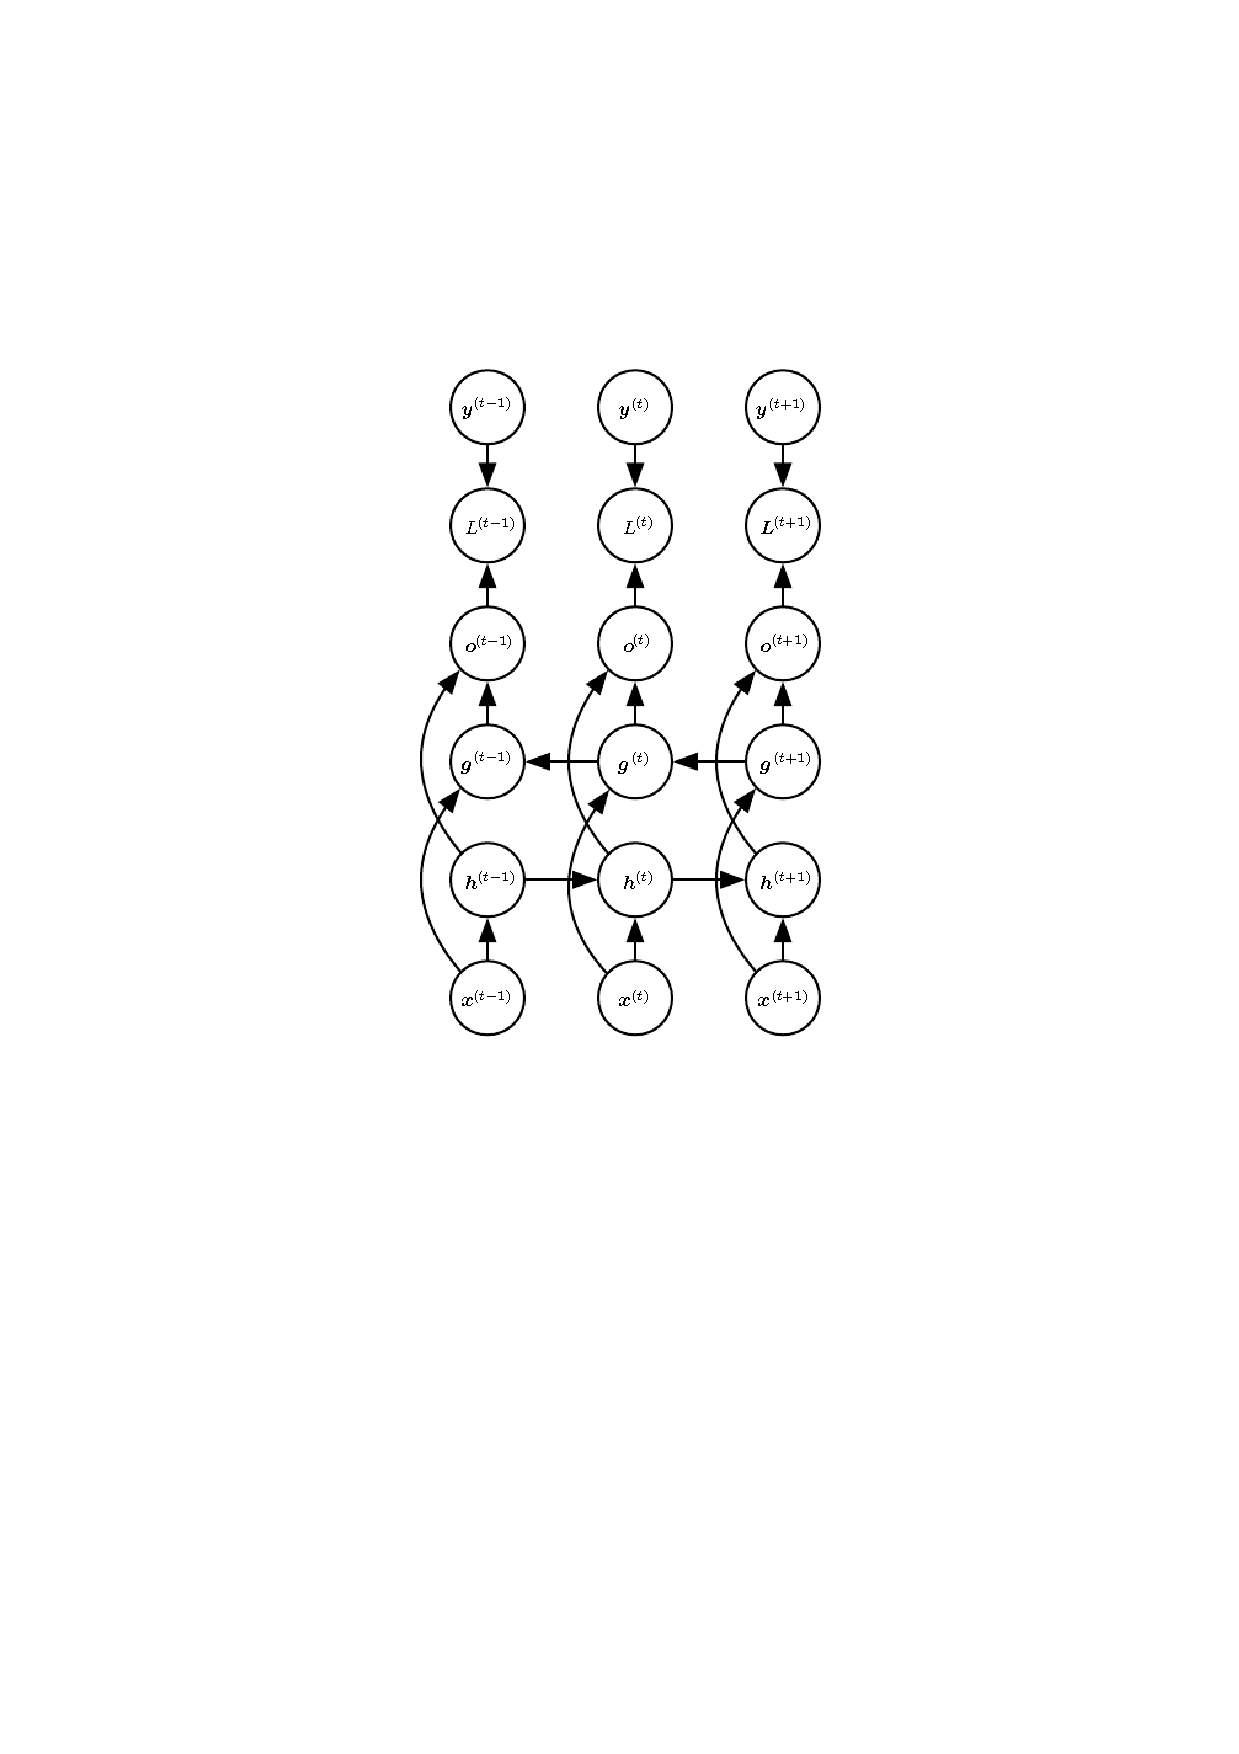
\includegraphics[width=0.6\textwidth]{../imgs/Bi-RNN.pdf}
\end{center}
\begin{itemize}
    \item $\egvh{t}$: state of the sub-RNN that moves forward through time
    \item $\egvg{t}$: state of the sub-RNN that moves backward through time
    \item $\egvo{t}$: compute a representation that depends on both the past and the future but is most sensitive to the input values around time $t$
\end{itemize}

\paragraph{Motivation}
\begin{itemize}
    \item The prediction $\egvy{t}$ may depend on the whole input sequence.
\end{itemize}

\paragraph{Applications}
\begin{enumerate}
    \item{In speech recognition, handwriting recognition and many other sequence-to-sequence learning tasks: \\
        The correct interpretation of the current sound as a phoneme may depend on the next few phonemes because of co-articulation and may even depend on the next few words because of the linguistic dependencies between nearby words.
    }
\end{enumerate}

\paragraph{Variants}
\begin{enumerate}
    \item{
        For two-dimensional input (such as images):
        \begin{itemize}
            \item Having four RNNs, each on going in one of the four directions
            \item At each point $(i,j)$ of a $2-D$ grid, an output $O_{i,j}$ could then compute a representation that would capture mostly local information but could also depend on long-range inputs.
            \item{
                Restrictions:
                \begin{enumerate}
                    \item Typically more expensive compared to a convolutional network.
                \end{enumerate}
            }
        \end{itemize}
    }
\end{enumerate}


\section{Encoder-Decoder or Sequence-to-Sequence Architectures}

The input to RNN is often called the "context". We want to produce a representation of this context, $C$. The context $C$ might be a vector or sequence of vectors that summarize the input sequence $\vX = (\egvx{1},\dots,\egvx{n_x})$.
The idea is as follow
\begin{itemize}
    \item An \textbf{encoder} or \textbf{reader} or \textbf{input} RNN processes the input sequence. The encoder emits the context $C$, usually as a simple function of its final hidden state $\vh_{n_x}$.
    \item A \textbf{decoder} or \textbf{writer} or \textbf{output} RNN is conditioned on that fixed-length vector to generate the ouput sequence $\vY = (\egvy{1},\dots,\egvy{n_y})$.
\end{itemize}
\begin{center}
    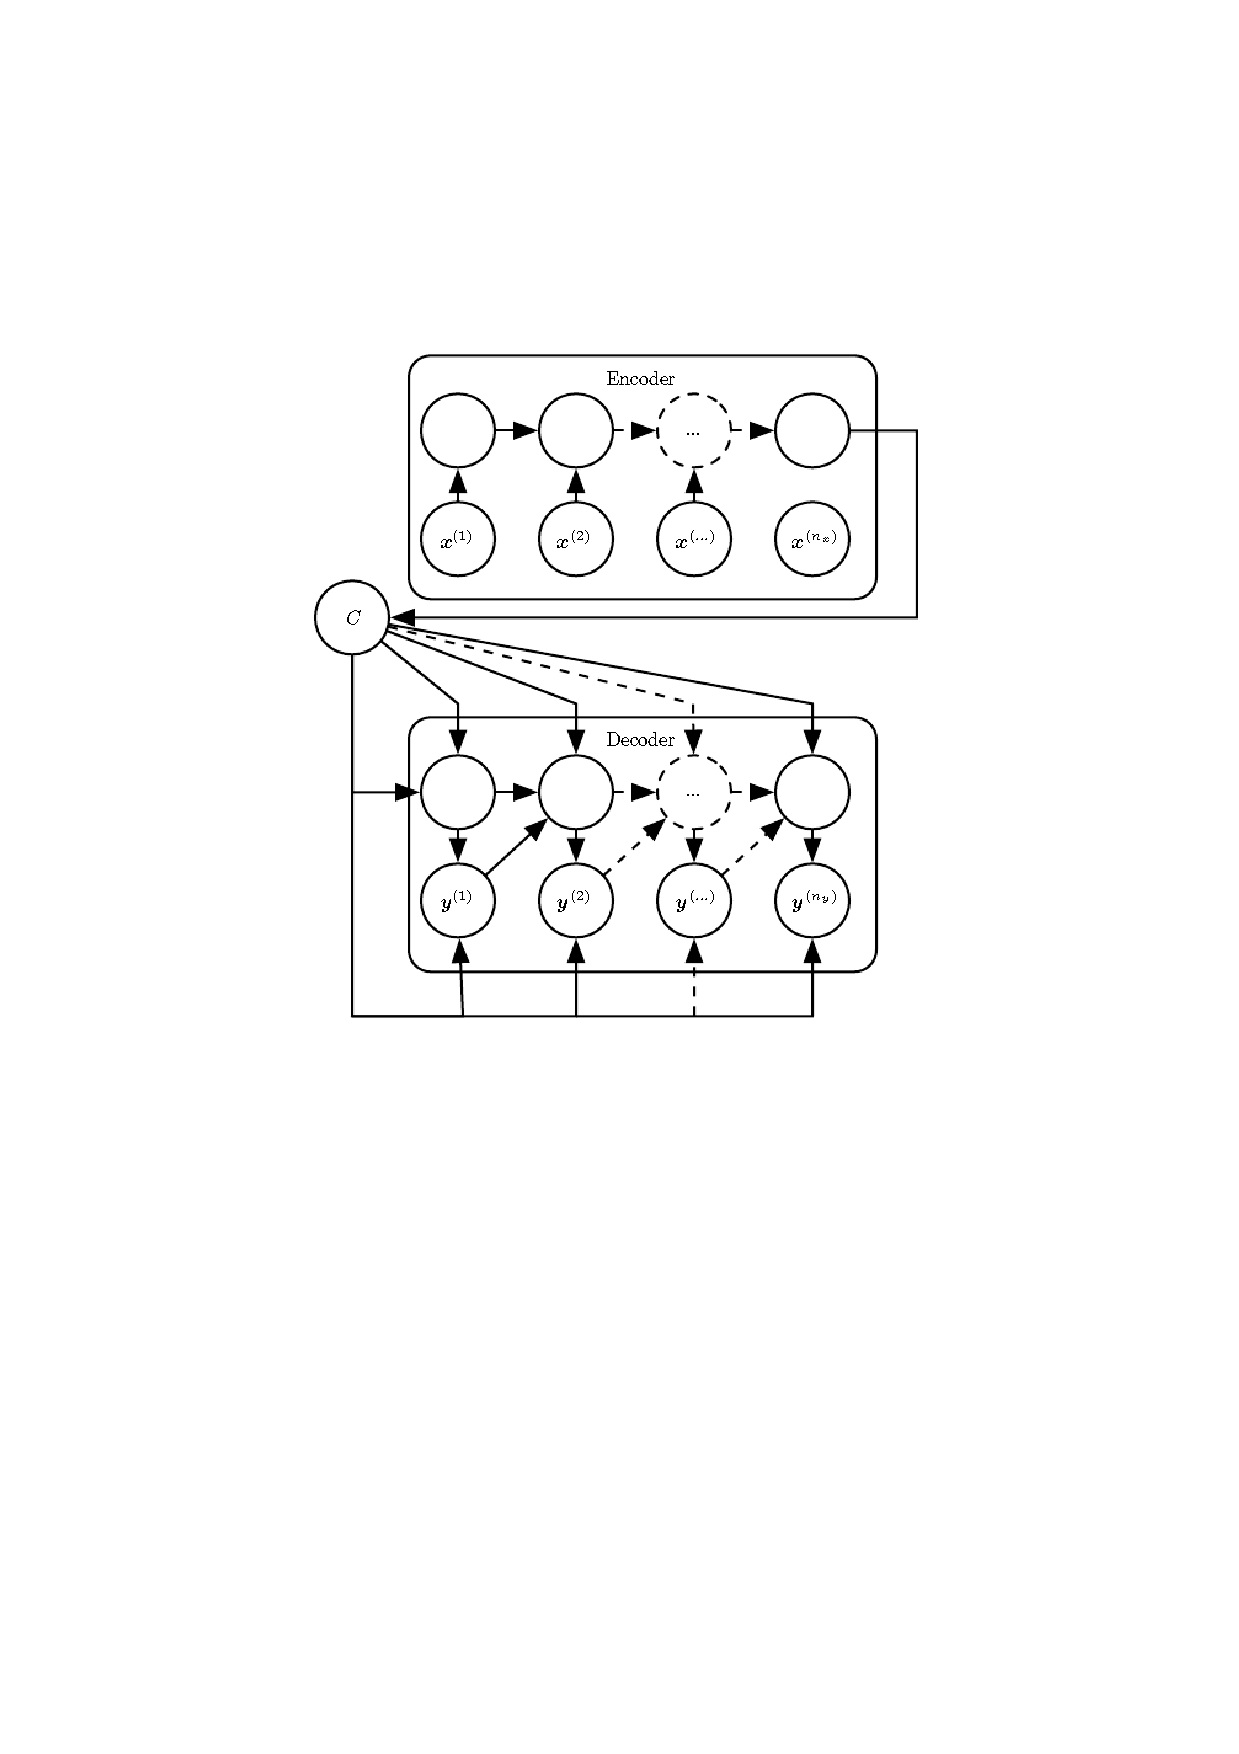
\includegraphics[width=0.8\textwidth]{../imgs/Seq2Seq.pdf}
\end{center}

\paragraph{Motivation}
\begin{itemize}
    \item Map an input sequence to an output sequence not necessarily of the same length.
\end{itemize}

\paragraph{Characteristics}
\begin{itemize}
    \item{
        Loss: The two RNNs are trained jointly to maximize the average of $\log P(\egvy{1},\dots,\egvy{n_y} \mid \egvx{1},\dots,\egvx{n_x})$ over all the pairs of $\vx$ and $\vy$.
    }
\end{itemize}

\paragraph{Applications}
\begin{enumerate}
    \item Speech recognition, machine translation, question answering.
\end{enumerate}

\paragraph{Restrictions}
\begin{itemize}
    \item If the context $C$ has a dimension that is too small to properly summarize a long sequence. (see \textbf{attention mechanisme} for solutions)
\end{itemize}


\section{Deeper RNNs}
A RNN can be deeper in many ways:
\begin{enumerate}
    \item The hidden recurrent state can be broken down into groups organized hierarchically.
    \item{
        Deeper computation (e.g., an MLP) can be introduced in three parts:
        \begin{enumerate}
            \item input-to-hidden
            \item hidden-to-hidden
            \item hidden-to-output
        \end{enumerate}
        This may lengthen the shortest path linking different time steps.
    }
    The path-lengthening effect can be mitigated by introducing skip connections.
\end{enumerate}
\begin{center}
    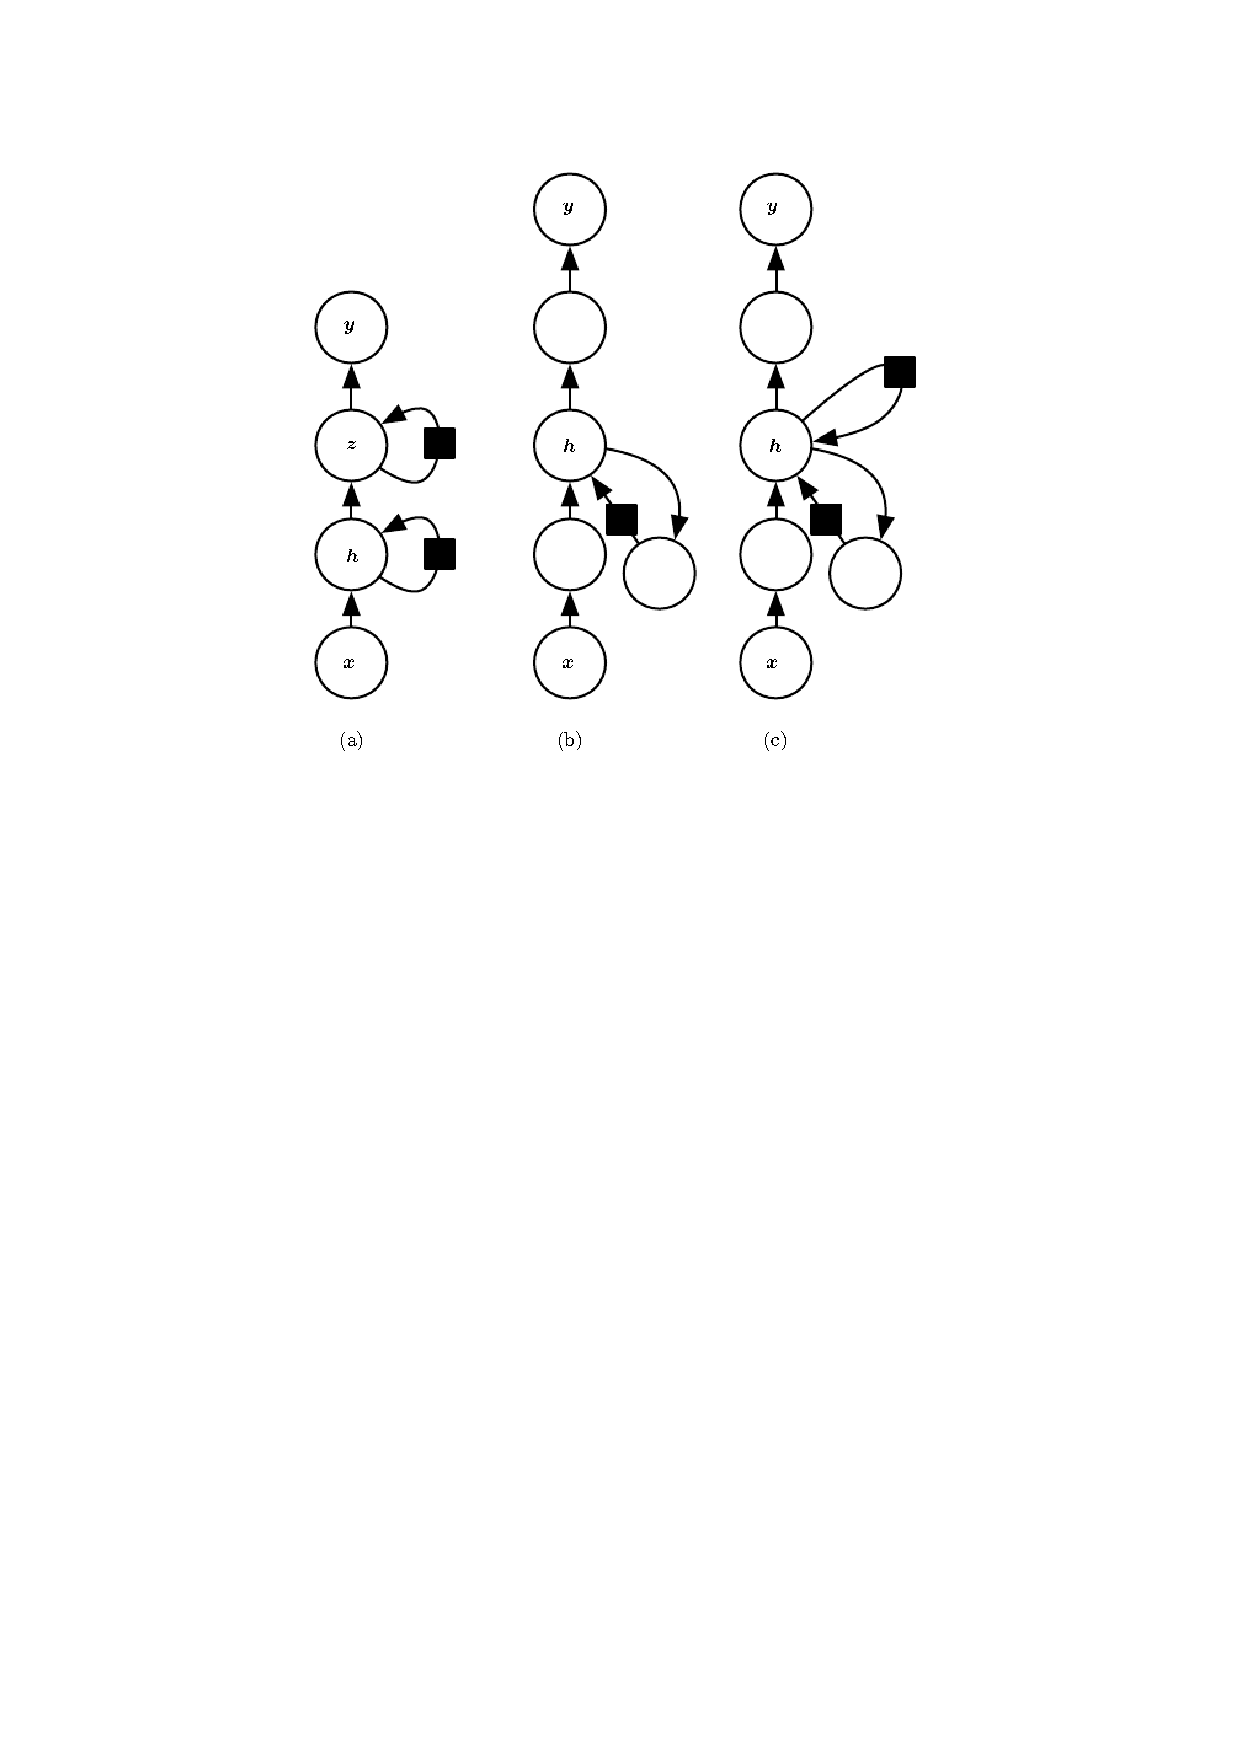
\includegraphics[width=0.8\textwidth]{../imgs/Deeper_RNNs.pdf}
\end{center}


\section{Attention Mechanism}

Read the whole sentence or paragraph (to get the context and the gist of what if being expressed), then produce the translated words one at a time, each time focusing on a different part of the input sentence to gather the semantic details required to produce the next output word.
\newline
The attention-based system used to focus on specific parts of the input sequence at each time step has three components:
\begin{enumerate}
    \item A process that reads raw data (such as source words in a source sentence) and converts them into distributed representations, with one feature vector associated with each word position.
    \item A list of feature vectors storing the ouput of the reader. This can be understood as a memory containing a sequence of facts, which can be retrieved later, not necessarily in the same order, without having to visit all of them.
    \item A process that exploits the content of the memory to sequentially perform a task, at each time step having the ability put attention on the content of one memory element (or a few, with a different weight).
\end{enumerate}
The third component generates the translated sentence.

\paragraph{Motivation}
\begin{itemize}
    \item{
        Using a fixed-size representation to capture all the semantic details of a very long sentence of, say, 60 words is very difficult.
        \begin{itemize}
            \item It can be achieved by training a sufficiently large RNN well enough and for long enough.
        \end{itemize}
    }
\end{itemize}

\paragraph{A modern attention mechanism}
\begin{center}
    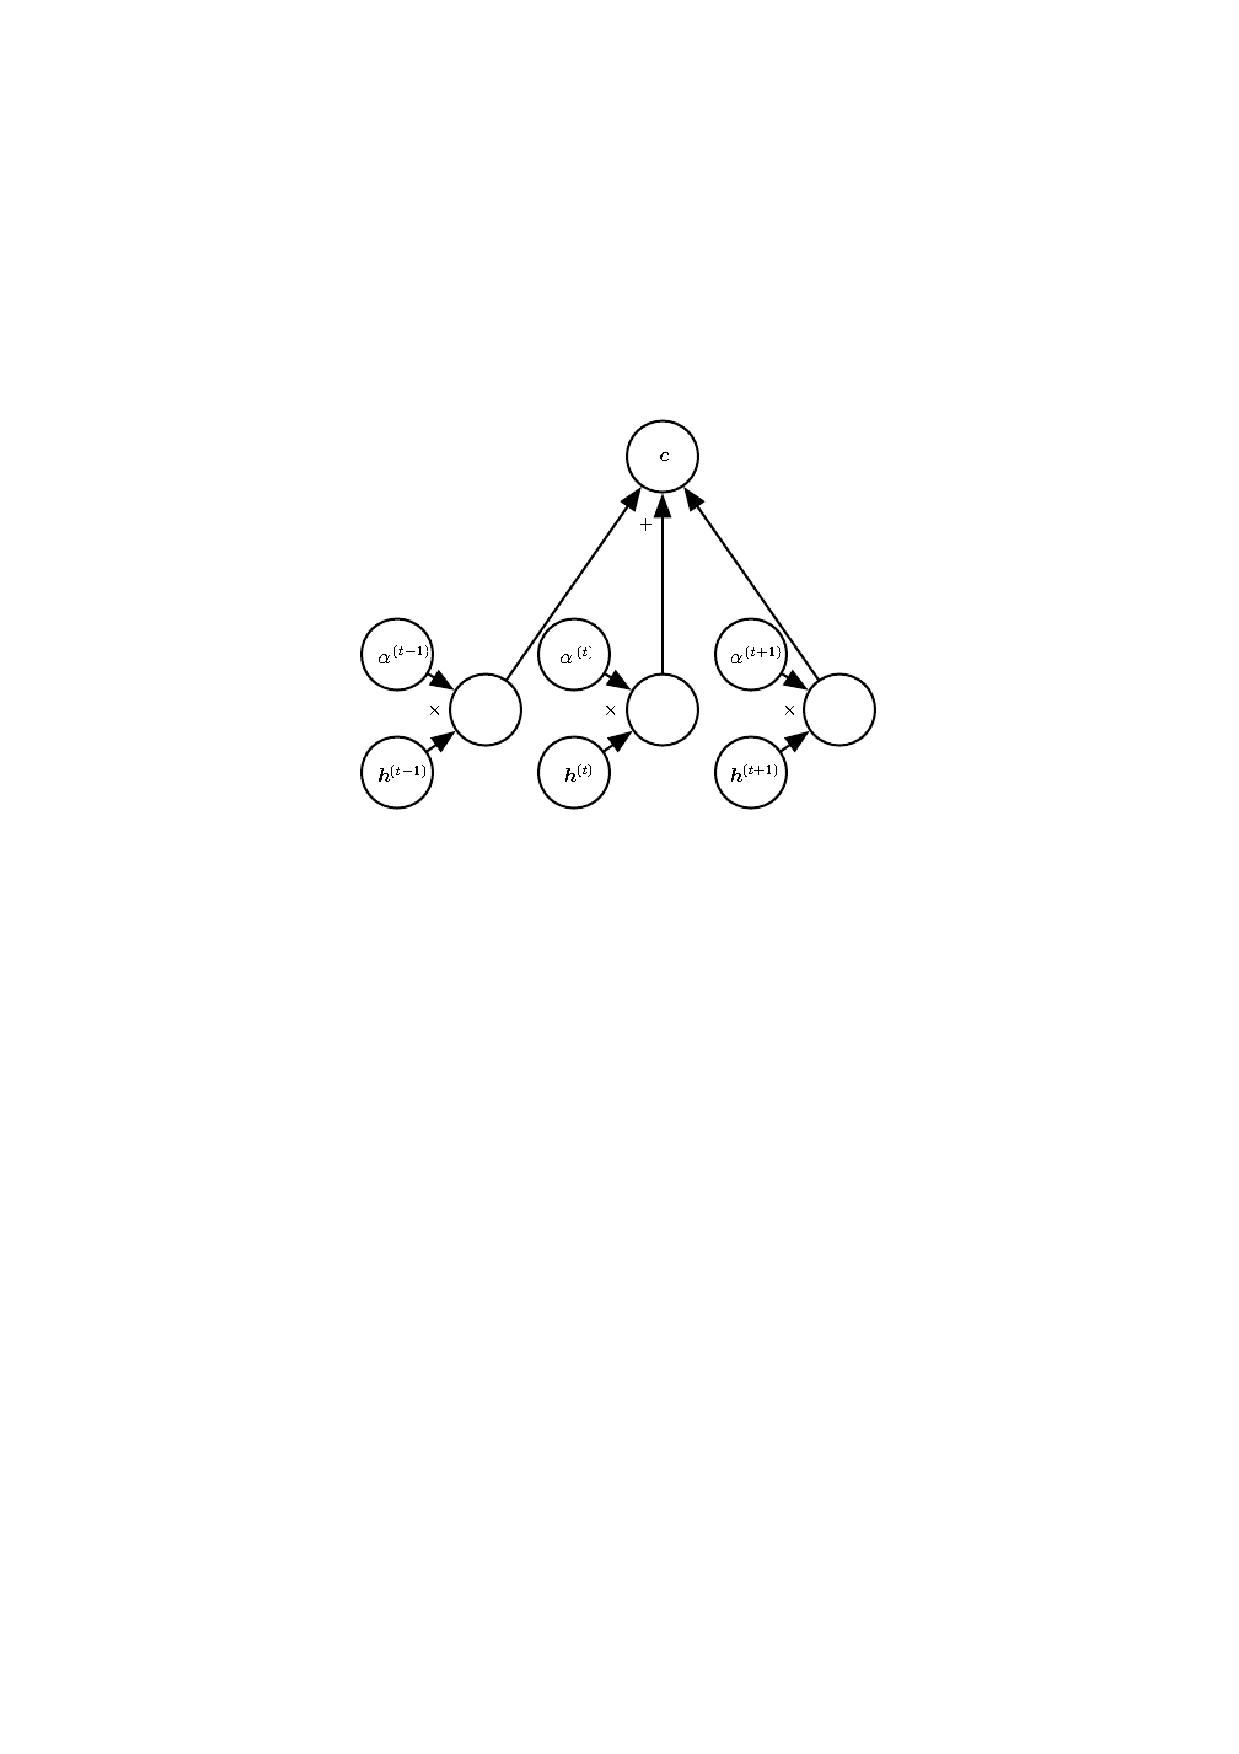
\includegraphics[width=0.8\textwidth]{../imgs/Attention_Mechanism.pdf}
\end{center}
\begin{itemize}
    \item A context vector $\vc$ is formed by taking aweighted average of feature vectors $\egvh{t}$ with weights $\alpha^{(t)}$.
    \item The feature vectors $vh$ may be hidden units of a neural network or raw input to the model.
    \item The weights $\alpha^{(t)}$ are produced by the model iteself. They are usually values in the interval $[0, 1]$ and are intended to concentrate around just one $\egvh{t}$ so that the weighted average approximates reading that one specific time step precisely. The weight $\alpha^{(t)}$ are usually produced by applying a softmax function to relevance scores emitted by another portion of the model.
    \item More expensive computationally than directly indexing the desired $\egvh{t}$, but direct indexing cannot be trained with gradient descent.
\end{itemize}


\end{document}